El proceso general del método propuesto se ilustra en la imagen \ref{fig:workflow}. El método consiste en determinar qué fragmentos deben unirse en la etapa de correspondencia, y ensamblarlos en la etapa de alineación. Este proceso se realiza de manera iterativa entre pares de fragmentos hasta que el objeto esté completo o no exista un par de caras fracturadas con un \textit{score} mayor a un \textit{threshold} definido. En las siguientes dos secciones se explica a detalle la etapa de correspondencia y alineación.
\begin{figure}[!h]
    \centering
     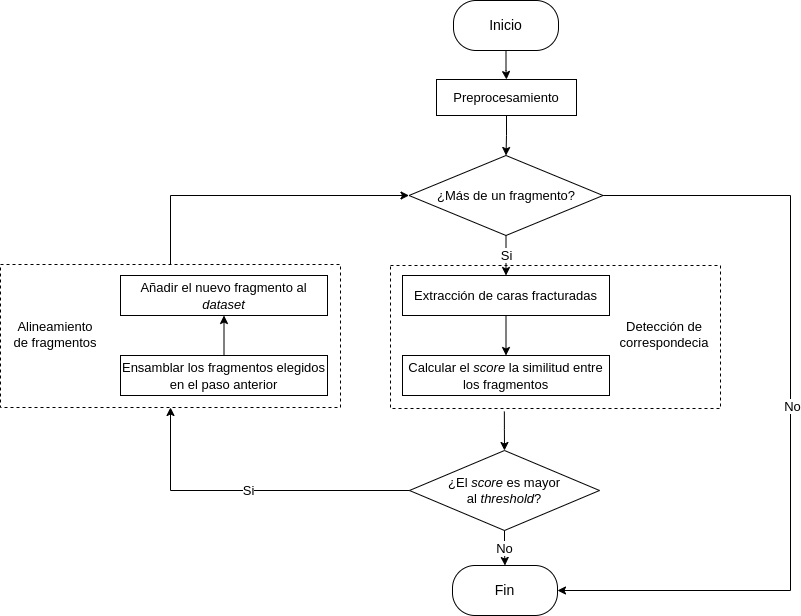
\includegraphics[scale=0.4]{images/workflow.png}
    \caption{Diagrama de flujo del método propuesto}
    \label{fig:workflow}
\end{figure}

\subsection{Correspondencia}
La etapa de correspondencia inicia con la extracción de las caras fracturadas de los fragmentos 3D. Luego, se calcula el \textit{score} de similitud entre caras de diferentes fragmentos. Finalmente, se selecciona la pareja de fragmentos con el mayor \textit{score} entre caras fracturadas para que sean la etrada de la siguiente etapa.

\subsubsection{Extracción de caras fracturadas}
La extracción de caras fracturadas se realiza sobre cada fragmento y es un proceso compuesto por tres pasos. Primero, se extraen los \textit{key points} del fragmento basado en su curvatura, donde la curvatura $c_p$ en un punto $p$ está definido por la raíz del promedio de la curva principal máxima $k_1$ y la mínima $k_2$ como se muestra en la ecuación \ref{eq:46}.

\begin{equation} \label{eq:46}
    c_p = \sqrt{\frac{k_1^2 + k_2^2}{2}}
\end{equation}

Segundo, se obtiene las curvas de las caras fracturadas a través de un algoritmo de \textit{boundary tracking}. Básicamente, dado un \textit{key point} $p$ se busca el conjunto de puntos más cercanos en un radio $r$, los cuales si son compartidos por más de $n$ \textit{key points}, se convierten en parte del borde junto con los \textit{key points} iniciales. \\

Tercero, se eliminan los bordes para extraer las caras del fragmento mediante un algoritmo de agrupamiento, donde se seleccionan los puntos más cercanos para formar grupos que representan las caras. Después, se evalúa la curvatura promedio de los puntos de cada clúster para determinar cuáles son las caras fracturadas. 

\begin{figure}[!h]
    \centering
     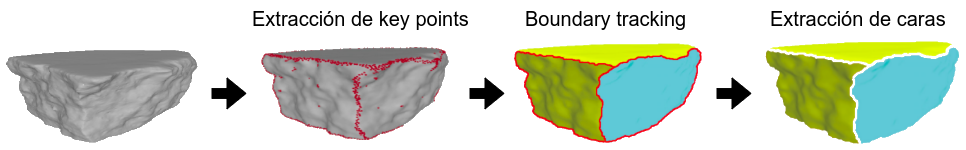
\includegraphics[scale=0.35]{images/fracture.png}
    \caption{Proceso de extracción de caras fracturadas}
    \label{fig:siamesa}
\end{figure}


\subsubsection{\textit{Score} de similitud}
El \textit{score} de similitud entre un par de caras fracturadas es obtenido por medio de una red siamesa como se muestra en la imagen \ref{fig:siamesa}. Primero, dos \textit{pointnets} extraen las características de las caras fracturadas $X$ y $Y$, donde los pesos son compartidos por ambas redes.  \\

Segundo, los vectores característicos $V_{X}$ y $V_{Y}$ se comparan y se obtiene el \textit{score} de similitud a partir de la ecuación \ref{eq:43}, la cual está dada por la tangente hiperbólica ($\tanh$) de la distancia euclidiana entre $V_{X}$ y $V_{Y}$. El objetivo de esta ecuación es obtener valores cercanos a 1 cuando la distancia es mínima, y valores cercanos a 0 en el caso contrario.

\begin{comment}
la distancia euclidiana es reemplazada por el coseno entre $V_{X}$ y $V_{Y}$ para determinar si los vectores son opuestos (-1) y se pueden ensamblar. Dado que el $score$ se encuentra entre 0 y 1, transformamos el resultado del coseno para que 1 represente que dos vectores se corresponden. 
\end{comment}

\begin{equation} \label{eq:43}
    score = \tanh\left(\frac{1}{||V_X - V_Y||_2}\right)
    % \qquad score = 1 - p
\end{equation}

Tercero, se utiliza el $score$ para calcular la función de pérdida de contraste descrita en la ecuación \ref{eq:45}, donde el primer término es diferente de cero si los vectores son similares, y el segundo término lo es si los vectores son diferentes. Nótese que $G$ es la etiqueta del \textit{ground truth} como se explicó en la subsección \hyperref[section:contrastive]{2.4.3}.

\begin{equation} \label{eq:45}
    loss = G * (1 - score)^2 + (1 - G) * score^2
\end{equation}

\begin{figure}[!h]
    \centering
     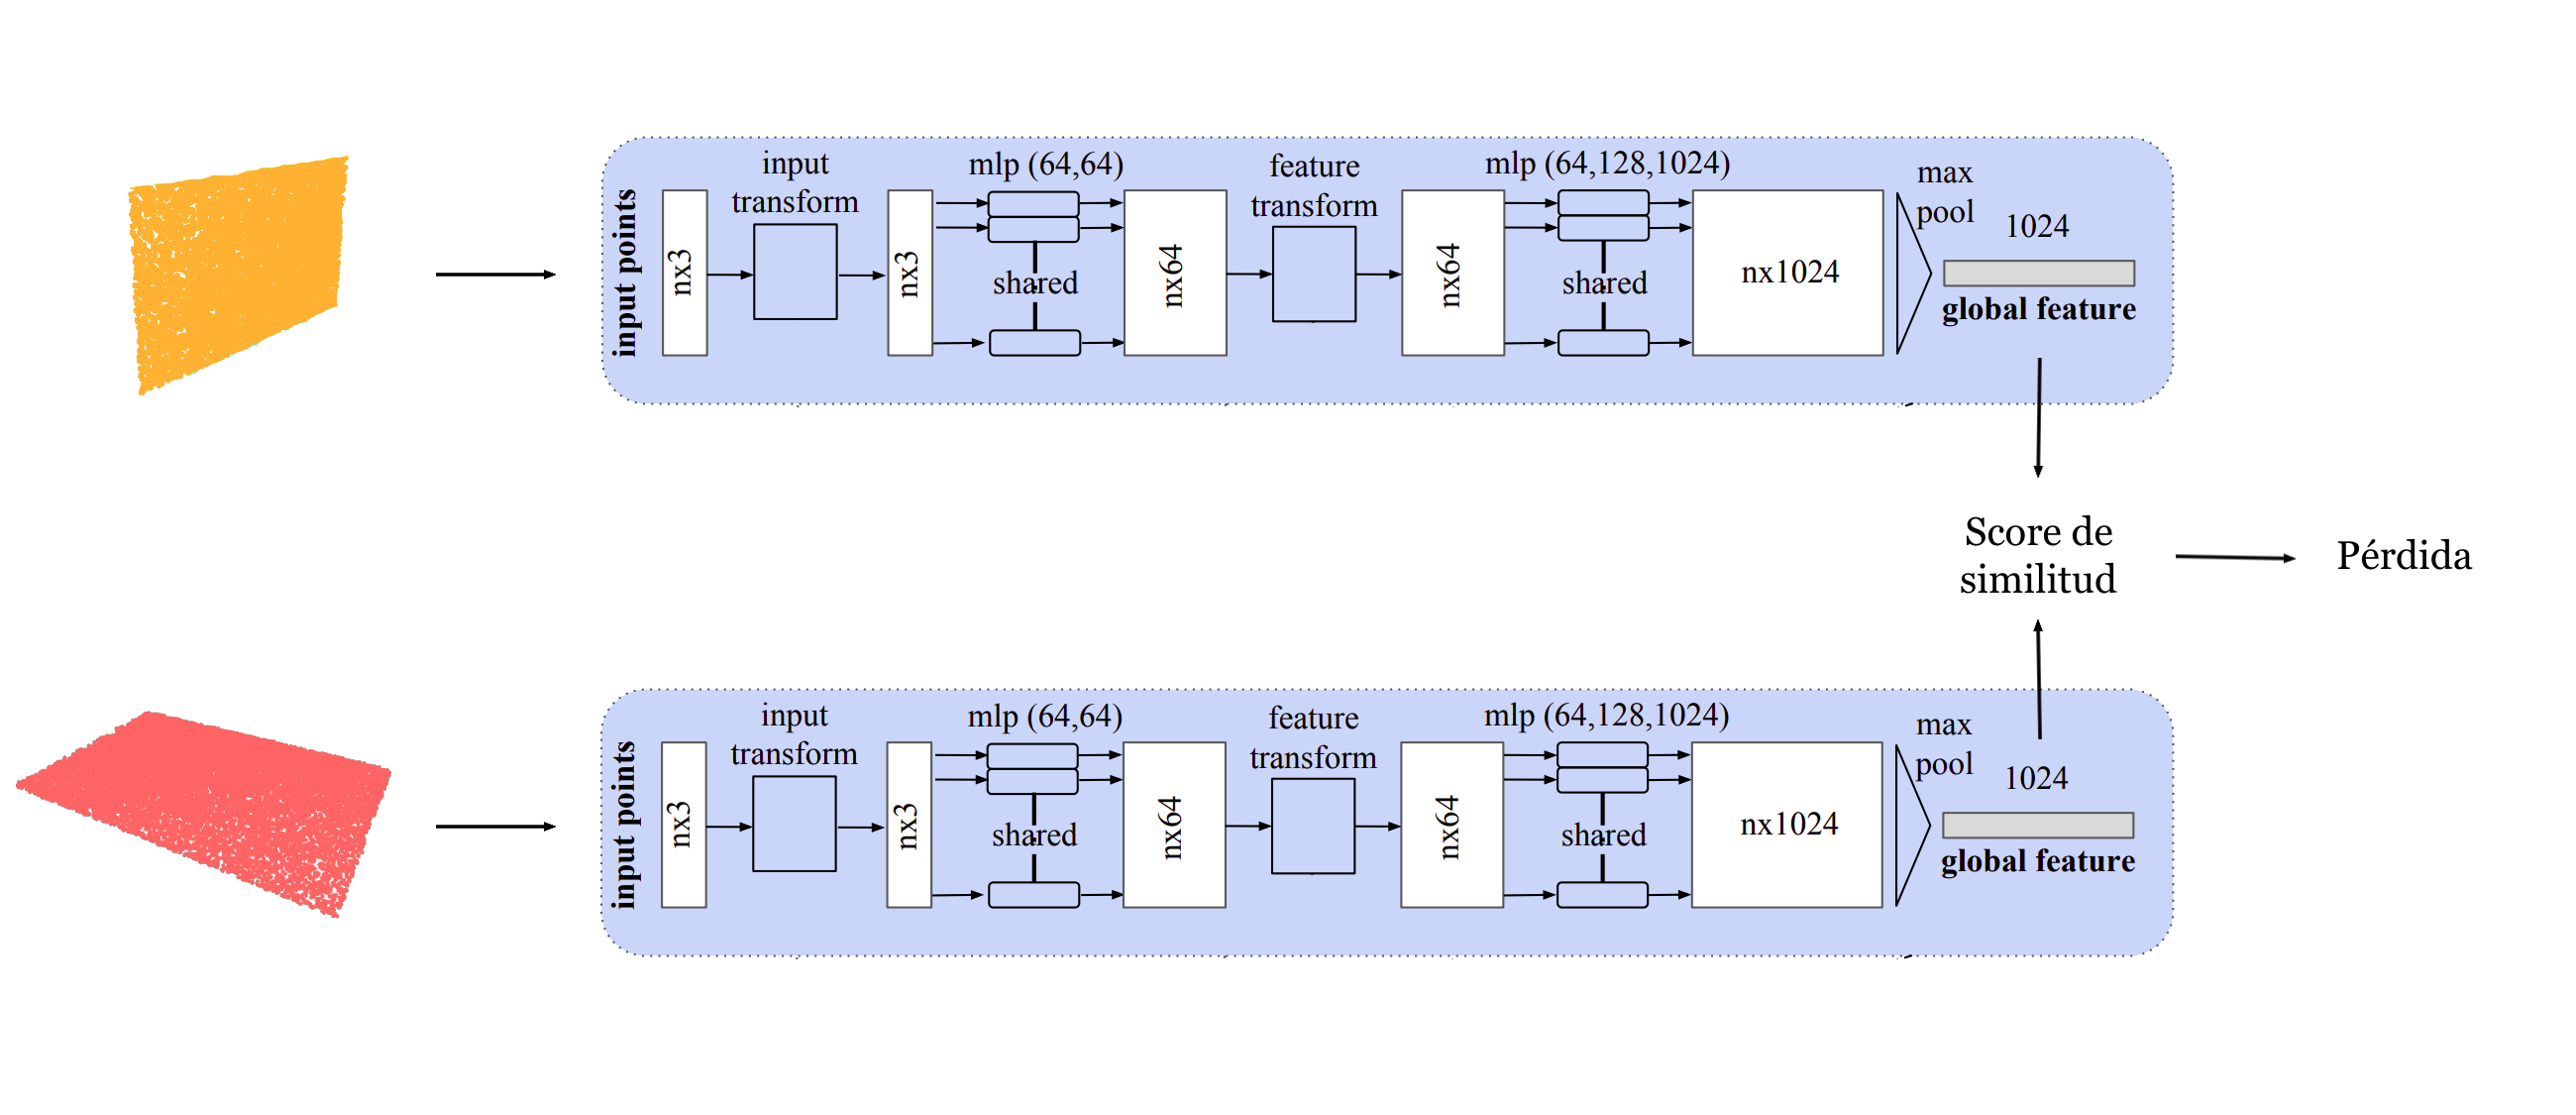
\includegraphics[scale=0.135]{images/siamesa.png}
    \caption{Arquitectura de la red de emparejamiento}
    \label{fig:siamesa}
\end{figure}


\subsection{Alineación}
La etapa de alineación ensambla los fragmentos obtenidos en el paso anterior y los convierte en un nuevo fragmento, el cual es añadido al \textit{dataset} original, y vuelve al paso de correspondencia.

\subsubsection{Ensamblaje de fragmentos}
El ensamblaje de fragmentos se realiza con el \textit{framework} de \textit{deep global registration (DGR)} \cite{10}. El \textit{framework} está compuesto por tres módulos principales: la extracción y predicción, el análisis de distribución balanceado, y la optimización final. La figura \ref{fig:dgr} ilustra los módulos mencionados a alto nivel.

\begin{figure}[!h]
    \centering
    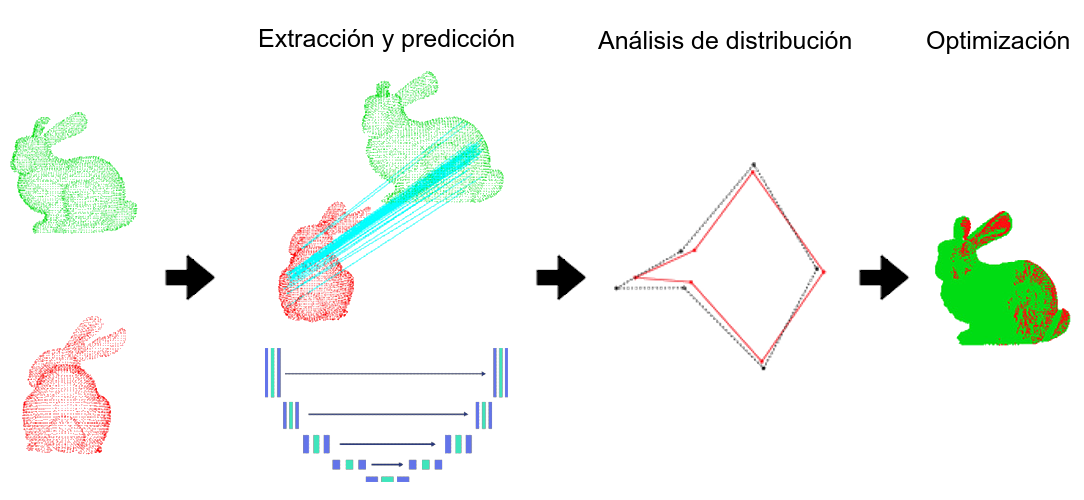
\includegraphics[scale=0.31]{images/registration.png}
    \caption{\textit{Pipeline} de DGR}
    \label{fig:dgr}
\end{figure}


Primero, el módulo de extracción y predicción tiene 3 etapas. En la primera, se extraen los vectores característicos de las nubes de puntos $X$ y $Y$. En la segunda, se genera un conjunto $M$ con las correspondencias $(x_i, y_i)$, donde $y_i$ es el vecino más cercano de $x_i$ en el espacio de vectores característicos. En la tercera, se utiliza una red neuronal convolucional (CNN) con estructura de U-net para predecir el \textit{likelihood} de las correspondencias del conjunto $M$. \\
    
Segundo, el módulo de análisis de distribución balanceado minimiza el error cuadrático medio ponderado entre los puntos de correspondencia (\ref{eq:1}), donde los pesos $w$ son el \textit{likelihood} obtenido en el módulo anterior. Este método genera un vector de rotación $\hat{R}$ y un vector de traslación $\hat{t}$. \\
\begin{equation} \label{eq:1}
    \argmin_{\hat{R}, \hat{t}}\frac{1}{N}\sum_{(i, j) \in M} w(i,j) ||x_{i} - (\hat{R}y_{j} + \hat{t})||^{2}
\end{equation}
    
Tercero, el módulo de optimización refina la alineación a través de la minimización de una función de pérdida robusta \ref{eq:2}. La función de filtrado $\phi$ en \ref{eq:50} selecciona los pesos mayores a $\tau$. La función $L(x, y)$ es la pérdida de Huber, la cual es menos sensible a los valores atípicos, y está descrita en \ref{eq:51}. Además, se utiliza un optimizador de descenso de gradiente como Adam o SGD para lograr la convergencia de los vectores de rotación $\hat{R}$ y traslación $\hat{t}$. \\
\begin{equation} \label{eq:2}
    loss = \sum_{i,j \in M} \phi(w(i,j)) \ L(x_i, \hat{R}y_{j} + \hat{t})
\end{equation}
\begin{equation} \label{eq:50}
    \phi(w) = I[w > \tau]
\end{equation}
\begin{equation} \label{eq:51}
    L(x, y) = 
    \begin{cases}
      \frac{1}{2}(x-y)^2 & para \ |x-y| \leq \delta \\
      \delta(|x-y| - \frac{1}{2}\delta) & otros 
    \end{cases} 
\end{equation}


\begin{comment}
Esta sección describe la propuesta metodológica. La metodología debe ser clara y debe tener un orden lógico. Ella debe tener relación con la problemática y los objetivos propuestos en la sub-sección Objetivos. Se debe tener en cuidado con los términos utilizados en esta sección. Ellos deberían haber sido descritos en el Marco Lógico. En esta parte también es usual colocar un diagrama o esquema que muestre el proceso que seguirán. 
\end{comment}
